%%%%This template was download from Canvas: MSc Projects/Modules/Latex/LatexDemoFiles.zip (https://canvas.bham.ac.uk/courses/56323/files/13146674?module_item_id=2600884)
%%%%%%%%%%%%%%%%%%%%% RJT TeX Template %%%%%%%%%%%%%%%%%%%%%
\documentclass[twoside,12pt,a4paper]{article}

%%%% BHAM PREAMBLE - SET THIS FIRST! %%%%
\newcommand{\bhamstudentname}{Nelson Quintanilla Castro}
\newcommand{\bhamthesistitle}{Analysing news articles about Russia’s war on Ukraine using Latent Dirichlet Allocation based topic modelling}
\newcommand{\bhamfronttitle}{Analysing news articles about Russia’s war on\\Ukraine using Latent Dirichlet Allocation\\ based topic modelling}
\newcommand{\bhamschool}{School of Computer Science}
\newcommand{\bhamcollege}{Engineering and Physical Sciences}
\newcommand{\bhamdegree}{MSc. Artificial Intelligence and Machine Learning}
\newcommand{\bhamid}{2291960}
\newcommand{\bhamsupervisor}{Dr Mohammed Bahja}
\newcommand{\bhamyear}{2022}
%%%%           %%%%

\usepackage[hyphens]{url}
\usepackage[breaklinks]{hyperref}
\usepackage{fancyhdr}
\usepackage[sort]{natbib} 
\usepackage{comment} % from http://www.latex-community.org/forum/viewtopic.php?f=5&t=4538
\usepackage{dirtree} % from http://blog.plenz.com/2011-07/represent-directory-structures-in-latex.html
\usepackage{longtable} % from http://stackoverflow.com/questions/2896833/how-to-stretch-a-table-over-multiple-pages
\usepackage{algorithm}   
\usepackage{algorithmic}   %both algorithm* from http://hasini-gunasinghe.blogspot.co.uk/2014/02/presenting-algorithmsprotocols-in-neat.html

\renewcommand{\algorithmiccomment}[1]{#1} %http://tex.stackexchange.com/q1uestions/61861/algorithmic-package-for-loop-and-comment-at-the-same-line

\pagestyle{fancy}
\renewcommand{\sectionmark}[1]{\markboth{#1}{}}	%from tex.stackexchange.com/questions/111361

\lfoot{\bhamstudentname}
\cfoot{}
\rfoot{}
\fancyhfoffset[L]{0cm} %this fixes the right page number margin issue.
\newcommand{\HRule}{\rule{\linewidth}{0.5mm}}
\renewcommand{\headrulewidth}{0pt}
\newcommand{\tab}{\hspace*{1.25em}}
\newcommand{\minitab}{\hspace*{0.25em}}

%footnote stuff
\usepackage{perpage}
\MakePerPage{footnote} %the perpage package command
\renewcommand*{\thefootnote}{\fnsymbol{footnote}}

\lhead{}\chead{}\rhead{}
\setlength{\headheight}{28pt} %fixes the warnings about headheight being too small
\setlength{\headsep}{6pt}
\pdfoutput=1 % we are running PDFLaTeX
\usepackage[left=3.65cm,right=2.7cm,top=4cm,bottom=4cm]{geometry}
\usepackage{titling}	
\setlength{\droptitle}{-2.75cm}   % This is your set screw\\
\usepackage{titlesec}
\titleformat*{\section}{\normalsize	\bfseries}
\titleformat*{\subsection}{\small \bfseries}
\titleformat*{\subsubsection}{\footnotesize \bfseries}
%modifies the size of the gaps between the top of the title and bottom
% arguments {type}{left}{top}{bottom}
\titlespacing*{\section} {0pt}{3ex plus 1ex minus .2ex}{2ex plus .2ex}
\titlespacing*{\subsection} {0pt}{2.25ex plus 1ex minus .2ex}{0.75ex plus .2ex}
\titlespacing*{\subsubsection}{0pt}{2.ex plus 1ex minus .2ex}{0.5ex plus .2ex}

\setlength{\intextsep}{0pt} %from http://tex.stackexchange.com/questions/25828/how-to-remove-change-the-vertical-spacing-before-and-after-an-algorithm-environ

\usepackage[pdftex]{graphicx}
\usepackage{enumitem}
\usepackage{pdfpages}
\usepackage{lastpage}
\usepackage{amsmath}
\usepackage{amsfonts}
\usepackage{amssymb}


\usepackage{epstopdf} %http://dirkraffel.com/2007/11/19/include-eps-files-in-latex/comment-page-2/

\usepackage{listings}
\lstset{
 basicstyle=\ttfamily,
  columns=fullflexible,
  keepspaces=true,
breaklines=true
} %from http://tex.stackexchange.com/questions/121601/automatically-wrap-the-text-in-verbatim

\newcommand{\todo}[1]{\textcolor{red}{TODO: #1}\PackageWarning{TODO:}{TODO found: #1!}} %from http://tex.stackexchange.com/questions/9796/how-to-add-todo-notes

\DeclareGraphicsExtensions{.jpg}
%%%%%%%%%%%%%%%%%%%%%  END of TEMPLATE %%%%%%%%%%%%%%%%%%%%%

\title{MSc. Project\\\bhamthesistitle}
\author{\textsf{\bhamstudentname}}

\date{}
\begin{document}

\pagenumbering{gobble} % fix at http://tex.stackexchange.com/questions/7355/how-to-suppress-page-number
% this came from http://en.wikibooks.org/wiki/LaTeX/Title_Creation and http://tex.stackexchange.com/questions/14778/error-with-hrule
\begin{titlepage}
\begin{center}
% this was from http://tex.stackexchange.com/questions/7219/how-to-vertically-center-two-images-next-to-each-other
\begin{minipage}{6in}
  \centering
  \raisebox{-0.5\height}{
\includegraphics[width=1.25in]{crest}}
  \hspace*{.2in}
  \raisebox{-0.5\height}{
\includegraphics[height=0.9375in]{uni}}
  \end{minipage}
  \\ [1.0cm]
\textsc{{\LARGE \bhamschool\\}College of \bhamcollege}\\[3.5cm]

\textsc{\Large MSc. Project}\\[0.5cm]

% Title
\HRule \\[0.4cm]
\begin{center}\Huge
\bhamfronttitle
\end{center}
\HRule \\[1.5cm]
% Team and Members

\begin{center}
Submitted in conformity with the requirements\\ for the degree of \bhamdegree\\
\bhamschool\\ University of Birmingham\\
\vspace{2cm}
\bhamstudentname\\
Student ID: \bhamid\\
Supervisor: \bhamsupervisor      
\end{center}
\vfill

% Bottom of the page
{\large September \bhamyear}

\end{center}
\end{titlepage}
\cleardoublepage

% Table of contents
\maketitle
\vspace{-5.5em} %fixes distance between \maketitle and the TOC
\begingroup
    \fontsize{9pt}{11pt}\selectfont
\tableofcontents
\endgroup

\clearpage
\phantomsection
\section*{Table of Abbreviations}
\begin{itemize}[nolistsep]
\item LDA -- Latent Dirichlet Allocation
\item API -- Application Programming Interface
\item NLTK -- Natural Language Toolkit
\item BOW -- Bag of Words
\end{itemize}
\addcontentsline{toc}{section}{Table of Abbreviations}

% List of Figures
\addcontentsline{toc}{section}{List of Figures}
\listoffigures

% List of Tables
\addcontentsline{toc}{section}{List of Tables}
\listoftables

\clearpage
% set up the page numbering and counter - Table of Abbreviations has no page number
% also set up the footers and headers appropriately.
\pagenumbering{arabic}
\setcounter{page}{1}
\lhead{}\chead{MSc. Project Report :: \nouppercase{Section \thesection\minitab :: \leftmark}}\rhead{}
\rfoot{Page \thepage \hspace*{0.2pt} of \pageref{LastPage}}
\renewcommand{\headrulewidth}{0.4pt}

\section{Overview}

\subsection{Abstract}
Lorem ipsum dolor sit amet, consectetur adipiscing elit, sed do eiusmod tempor incididunt ut labore et dolore magna aliqua. Ut enim ad minim veniam, quis nostrud exercitation ullamco laboris nisi ut aliquip ex ea commodo consequat. Duis aute irure dolor in reprehenderit in voluptate velit esse cillum dolore eu fugiat nulla pariatur. Excepteur sint occaecat cupidatat non proident, sunt in culpa qui officia deserunt mollit anim id est laborum.

\subsection{Acknowledgements}
This work could not have been possible without the academic support from Dr Mohammed Bahja and Dr Felipe Orihuela-Espina.

Dr Mohammed Bahja always motivated me and academically advised me how to approach many challenges during the dissertation process.

Dr Felipe Orihuela, who also was my tutor during the academic year of my Master's degree, was fundamental for me to get a better sense of how the UK education system works and how to better approach challenges but most importantly how to always strive for excellence even during hard times or in adversity.

\clearpage
\section{Introduction}
The ongoing conflict between Russia and Ukraine is a topic of pivotal importance not only for the protagonist's regions but also for the whole world. This war is already causing many negative economic, political, and social consequences on a different scale for many countries \citep{caldara_effect_2022}. As a result, this has become of paramount concern for governments and, subsequently for all types of media.

This is why there is currently a tremendous amount of information that has been generated about the Russo-Ukrainian conflict and there is no systematic way to analyse this corpora to examine what is currently happening regarding this conflict, to discover the main themes contained within it, and possibly draw conclusions about it.

At the same time, it is not humanly possible to read and study large quantities of articles with this thematic in a short period of time. To do this, experts in machine learning have created probabilistic topic modelling, a collection of several algorithms which are used to identify and interpret sizeable sets of documents that contain topical information. We can use topic modelling to identify the primary ideas that run through a sizable and otherwise unstructured collection of papers. We can arrange the collection in accordance with the themes found by applying topic modelling \citep{blei_probabilistic_2012}.

For the purpose of this work, latent dirichlet allocation (LDA) is going to be the topic modelling algorithm of choice. A collection of texts can be broken down into their key topics using LDA, where a topic is defined as a probability distribution over a vocabulary \citep{blei_latent_nodate}.

A set number of topics are proposed by LDA, and it is assumed that each document in a collection of documents reflects a combination of those themes. Under these presumptions, probabilistic inference techniques identify an embedded theme structure in a document collection. LDA offers a technique to easily summarise, peruse, and search huge document collections with this structure \citep{blei_probabilistic_2010}.

The main motivation of this work is to capture the main themes or topics that can be found on news articles available on the internet that cover events related to Rusia’s war on Ukraine. This represents an important topic to study because there is a need to derive insightful information from this vast amount of news about the war that are being generated in mass all over the world.

Furthermore, it is of utter importance to observe and detect significant patterns that are being communicated to the general public through news articles so we can predict consequences of the current state of the situation on the short term such as the economical, political, and social impact on human lives.

In this paper we provide an analysis of news articles retrieved from The Guardian newspaper that cover events related to the Russian invasion of Ukraine by utilising LDA based topic modelling with the purpose of obtaining abstract topics within a corpora of news articles. We also offer a way to assess the effectiveness and outcomes of our model. Additionally, we present the validation of our model by comparing it against human judgement. In order to allow others to duplicate our findings, we have also made our data sets publicly available. Further to this, we use pyLDAvis to interpret the topics obtained by our model in a more comprehensible and visual way. This software offers a global view of the topics and how they differ from one another while also enabling a close examination of the terms most closely associated with each specific topic \citep{sievert_ldavis_2014}.

The structure of this paper is as follows. In section 3 we examine the most recent studies in this field. In Section 4 we present the specifics of our approaches, including a description of data extraction, preprocessing, parameter tuning of our model, and evaluation metrics implemented. We provide our findings and engage in a discussion in Section 5. The discussion is presented in part 6, and our conclusion is presented in section 7.

\clearpage
\section{Literature Review}
\subsection{Subsection}
Lorem ipsum dolor sit amet, consectetur adipiscing elit, sed do eiusmod tempor incididunt ut labore et dolore magna aliqua. Ut enim ad minim veniam, quis nostrud exercitation ullamco laboris nisi ut aliquip ex ea commodo consequat. Duis aute irure dolor in reprehenderit in voluptate velit esse cillum dolore eu fugiat nulla pariatur. Excepteur sint occaecat cupidatat non proident, sunt in culpa qui officia deserunt mollit anim id est laborum.

\subsection{Subsection}
Lorem ipsum dolor sit amet, consectetur adipiscing elit, sed do eiusmod tempor incididunt ut labore et dolore magna aliqua. Ut enim ad minim veniam, quis nostrud exercitation ullamco laboris nisi ut aliquip ex ea commodo consequat. Duis aute irure dolor in reprehenderit in voluptate velit esse cillum dolore eu fugiat nulla pariatur. Excepteur sint occaecat cupidatat non proident, sunt in culpa qui officia deserunt mollit anim id est laborum.

\clearpage
\section{Methodology}
In this section we explain the steps we took in order to build and prepare our dataset, the model generation and parameter tuning process, methods of evaluation for our model, and lastly visualisation and interpretation of our resulting topics. The Figure \ref{fig:method_1} summarises the method we just mentioned.\\

\begin{figure}[h]
\centering
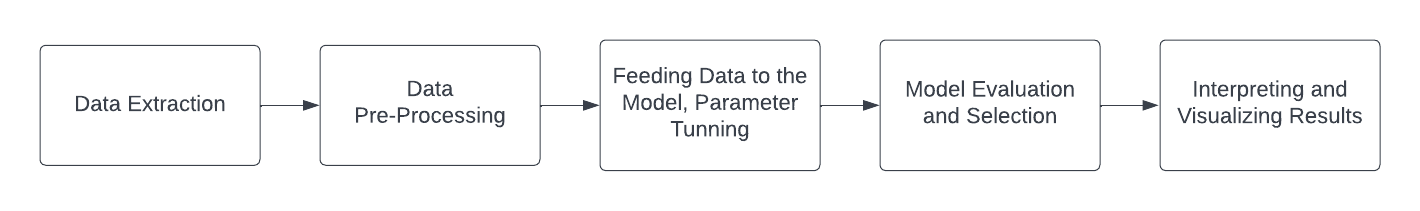
\includegraphics[scale=0.6]{method_1.png}
\caption{\textit{Diagram that summarises steps taken during the development of our work.}}
\label{fig:method_1}
\end{figure}

\subsection{Data Extraction}
To obtain a significantly large dataset of reliable news articles related to the Russian invasion of Ukraine we decided to use The Guardian digital newspaper. The reasoning behind this decision is because The Guardian is one of the most trusted newspapers in the UK and Europe in terms of objective journalism \citep{matsa_western_2018}. Additionally, they provide The Guardian – Open Platform, which is their public web service or application programming interface (API) that provides free access to all of the content that the Guardian produces, organised by tags and sections \citep{noauthor_theguardian_nodate}. This is specially useful in our case because we need to filter the news to reduce noise in our data and have articles relevant to the ongoing conflict between Russia and Ukraine.

To narrow-down the retrieval of the articles, we requested published data between the 2nd of February of 2022 (day in which Russia invaded Ukraine) and the 31st of August of 2022. Additionally, we created a function to interact with the API and retrieve news articles filtered by search term and section. This is to avoid obtaining non relevant news; for instance, we used the section "world" to point to data classified in this category and not other categories such as "sports" or "lifestyle". Furthermore, we used 2 search terms: Ukraine and Russia. We obtained 2 different datasets corresponding to the mentioned search terms. After that, we merged both datasets and removed duplicates that could have existed in both to avoid redundancy. We also removed non pertinent articles that contained information about topics not related the conflict.

The resulting dataset is a json containing a list of 2275 news articles with their id, title of the article, body of the article, and url to read the article on the web. Such dataset is available in the repository included in Section~\ref{section:appendix} so it can be used for future research or work.

\subsection{Data Pre-Processing}
Before feeding the data to our model it is required to prepare the data \citep{jacobi_quantitative_2016}.

Following is a detailed description of the processes we took when completing the analysis for our case study. 

\subsubsection{Dataset Relevant Features}
Before starting pre-processing the data we display important features from our dataset, such as the number of articles to be used and the average word count per article. This is just to have a rough idea of the length of each document we are using for the purposes of training our model. In our case, we have a total of 2275 news articles and an average of 864 words per article.

\subsubsection{Normalisation and Tokenisation}
A topic model does not analyse documents directly; rather, it employs a so-called document–term matrix that is derived from the documents. This matrix displays the frequency for each term (word) in each document \citep{jacobi_quantitative_2016}. The initial step in the creation of this matrix is normalisation and tokenisation, for which each page is converted into a list of lowercase words, ignoring short and long words.

\subsubsection{Stop Word Removal}
Stop words are the words in a stop list that are filtered out prior to processing natural language data (text) due to their insignificance \citep{rajaraman_mining_2011}.

We compared three standard lists of stop words from extensively used libraries for machine learning applications: Natural Language Toolkit (NLTK) \citep{bird_natural_nodate}, scikit-learn \citep{pedregosa_scikit-learn_nodate}, and spaCy \citep{spacy2}. There is a file dedicated to do this comparison on our repository included in Section~\ref{section:appendix}. However, it is worth mentioning that our final decision was to merge the lists of stop words since this leads to better results in terms of removing words that are not adding any meaning, for instance "but", "end", and "the".

\subsubsection{Lemmatisation}
Lemmatisation is an important part of the preprocessing of the data. It reduces all words to their "lemma" by the use of a lexicon and regular conjugation rules. Thus, lemmatization reduces "is" and "were" to their respective lemma (to be) "be" \citep{jacobi_quantitative_2016}. There is also another technique called stemming which removes the endings of the words leaving just the "stems". Using the commonly employed Porter stemming algorithm, for instance, "weaknesses" becomes "weak" while "failures" and "failure" both become "failur" \citep{jacobi_quantitative_2016}. 

In our case lemmatisation was preferred over stemming because it produced better results as compared to stemming which sometimes returned words that were missing letters at the end and therefore did not exist in the English dictionary.

For the analysis presented here we used the lemmatiser from spaCy \citep{spacy2} which which assigns tokens' base forms using criteria derived from part-of-speech tags (POS).

\subsubsection{Transforming the documents in a vectorised form (Bag of Words Representation)}
As we mentioned earlier, before we feed the data to the model we need to transform the documents into a document-term matrix. This way of expressing our dataset is known as Bag of Words (BOW) representation. BOW represents the content of the documents by showing the frequency of the word on every document. Once we have this, we are ready to start training our model.

After using the aforementioned strategies, we have removed a number of terms from our initial tokenised dataset and adjusted the remaining words' structure to make them more effective for training our model. In the following section, we are going to delve into the model training and tunning.

\subsection{Model Training and Parameter Tunning}
There are numerous tools available for Topic modelling and analysis, including professional and amateur software, commercial and open-source software. Some examples of these well known tools that have been used by a large number of scholars in the past are Mallet \citep{McCallumMALLET}, TMT \citep{2009-topic-modeling-social-sciences}, and Gensim \citep{jelodar_latent_2019}.

For the training of our model we used Gensim, which is a Python package that provides algorithms for Latent Dirichlet Allocation that are memory-efficient, scalable, and quick \citep{rehurek_gensimstatistical_nodate, Rehurek10softwareframework}.

In order to train our LDA model we need to provide it with different parameters as it can be observed in Figure~\ref{fig:lda_multicore}. From all the parameters, one of the most important ones is the number of topics we want to extract from our dataset as this one affects greatly on the quality of the results. Furthermore, choosing the number of topics in LDA is typically determined by assessing the perplexity of numerous models built with varying values of number of topics as a parameter and choosing the one with the lowest perplexity value \citep{blei_probabilistic_2010}.

Perplexity is a metric for evaluating language models, where a low score denotes a model with superior generalisation, as determined by \citep{asmussen_smart_2019, xu_probabilistic_2016, blei_correlated_2007, zhao_heuristic_2015}. 

Reducing the perplexity score is equivalent to increasing the chance of all articles belonging to a topic. The criteria for picking the optimal number of topics is to strike a balance between a manageable number of topics and the lowest possible level of perplexity. The optimal amount of topics can vary substantially depending on the purpose of the analysis. As a general guideline, fewer topics are utilised for a general overview, while more topics are used for a more detailed look \citep{asmussen_smart_2019}. In our case, we geared our experimentation towards obtaining a general overview.

Coherence score is also extensively used in topic model experiments as an assessment tool \citep{li_seeded-btm_2019, ferner_automated_2020, albalawi_using_2020, towne_measuring_2016} and it indicates the degree of semantic similarity of high-scoring terms in the text and helps to differentiate the semantic interpretation of themes based on statistical inference \citep{ray_review_2019}.  

Having mentioned that, once we generated our corpus or Bag of Words representation of our dataset and our dictionary (a dictionary object that contains every single word on the entire dataset without duplicates), we created a function to generate many models at once with a different value of number of topics.

The first run we did was for models with 2, 8, 14, 20, 26, 32, and 38 number of topics. As we will explain further, we did several runs with different number of topics. At this point we computed the coherence score and perplexity for each of the models generated and as it can be observed in figure~\ref{charts_models}. We assessed the calculated perplexity and coherence and decided to do a second run for models with 2, 4, 6, 8, 10, 12, and 14 number of topics. 

We assessed the coherence and perplexity values, as well as the associated words with the highest probability for each of the topics of the generated models as it can be seen on Figure~\ref{fig:visualise_topics}, and based on that we started adding custom words to our list of stop words. The purpose of this is to avoid getting some of the words repeated in many topics (this is the case for words that occur in the majority of the documents). Therefore, we removed the following words: Ukraine, Ukrainian, Russia, Russian; and ran our model a third time. 

We assessed again the metrics in addition to the associated words for each of the topics of the model generated and this time we removed the following words: war, people, city; and ran our model a fourth time.

Lastly, we assessed in a similar manner, removed the words: country, year, day; and ran our model a fifth time.

For each of the runs in the process previously described we also did several other runs to tune the remaining parameters of the model by trial and error. When the results were better, we continued with the next iteration of runs. In the end, we selected the 3 best models from the last run. From these 3 models, we are going to find out which one is the best one utilising human judgement metrics.\\

\begin{figure}[h]
\centering
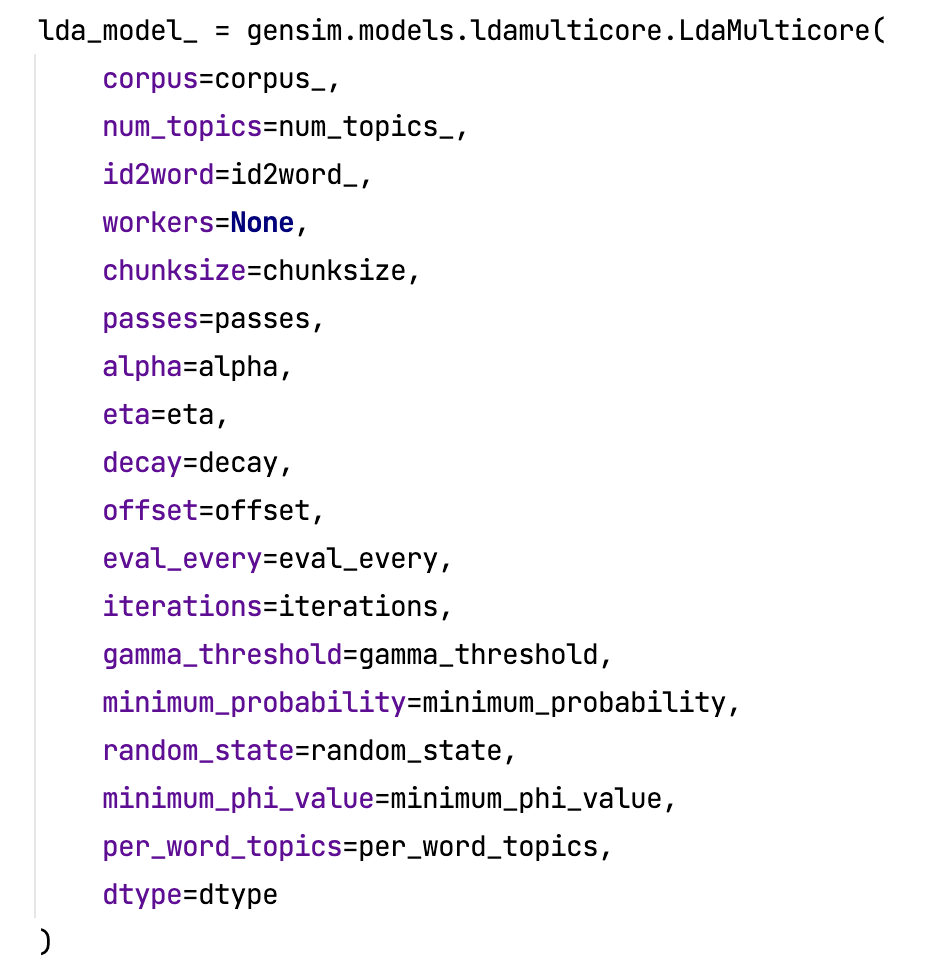
\includegraphics[scale=0.45]{lda_multicore.png}
\caption{\textit{LdaMulticore function from Gensim to train or LDA model.}}
\label{fig:lda_multicore}
\end{figure}

\begin{figure}[h]
\centering
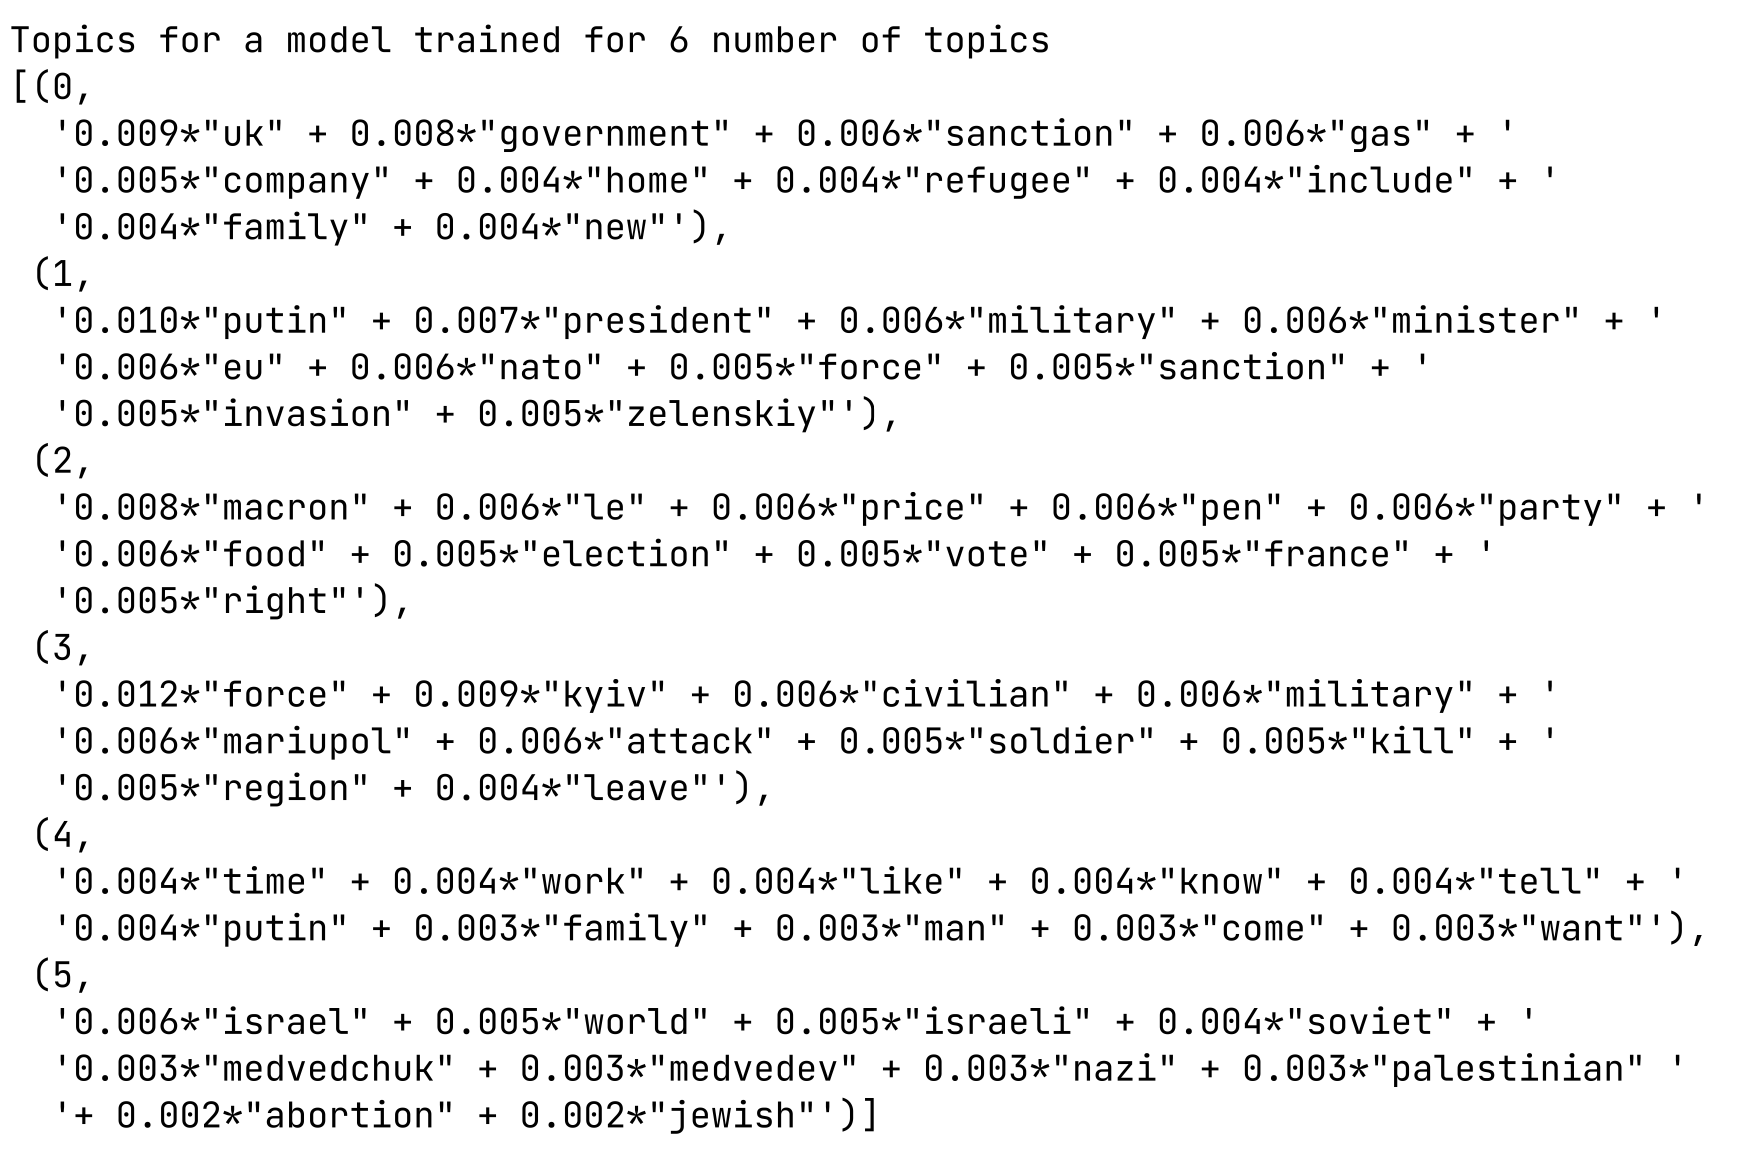
\includegraphics[scale=0.4]{visualise_topics.png}
\caption{\textit{Visualising topics and their 10 highest probable keywords for a model generated with 6 number of topics}}
\label{fig:visualise_topics}
\end{figure}

\subsection{Model Evaluation and Selection}
To further evaluate our models we used human judgement metrics as well. We employ two tasks to build a formal environment in which humans can evaluate the two components of a topic model's latent space. The first element is the composition of the topics. We construct a task to determine whether a topic has semantic coherence that is human-identifiable. This activity is known as word intrusion, as participants must recognise a fictitious word that has been put into a topic. The second assignment evaluates the validity of the relationship between a document and a topic. This task is known as topic incursion because the subject must identify a topic that the model did not correlate with the document \citep{nikolenko_topic_2017}.

In Figure~\ref{fig:forms_results} it can be observed the human tasks we provided for 10 users to answer. The purpose of these tasks was to select the best model amongst the three best models we picked in the last step. For each model, in total, each user responded to 5 word intrusion challenges and 3 topic intrusion challenges. The url to the questionary can be found in the repository included in Section~\ref{section:appendix}. Responses are no longer accepted but you can see the results.

To create the questionnaire, we used the 3 models in 3 news articles. For the word intrusion task, six words are presented to the individual in a random order.
The user's objective is to identify the word that does not belong with the others, also known as the intruder. Five of the six words correspond to the highest probable words from a topic but the sixth word is an intruder \citep{nikolenko_topic_2017}..

The topic intrusion challenge examines if a topic model's breakdown of documents into a variety of subjects corresponds to human evaluations of the document's content \citep{nikolenko_topic_2017}. 

Both experiments were made in a similar fashion to \citep{nikolenko_topic_2017, chang_reading_nodate}. Word and topic intruders were selected at random from terms and topics not present in the topic and text, respectively, similar to \citep{nikolenko_topic_2017}.

\begin{figure}[h]
\centering
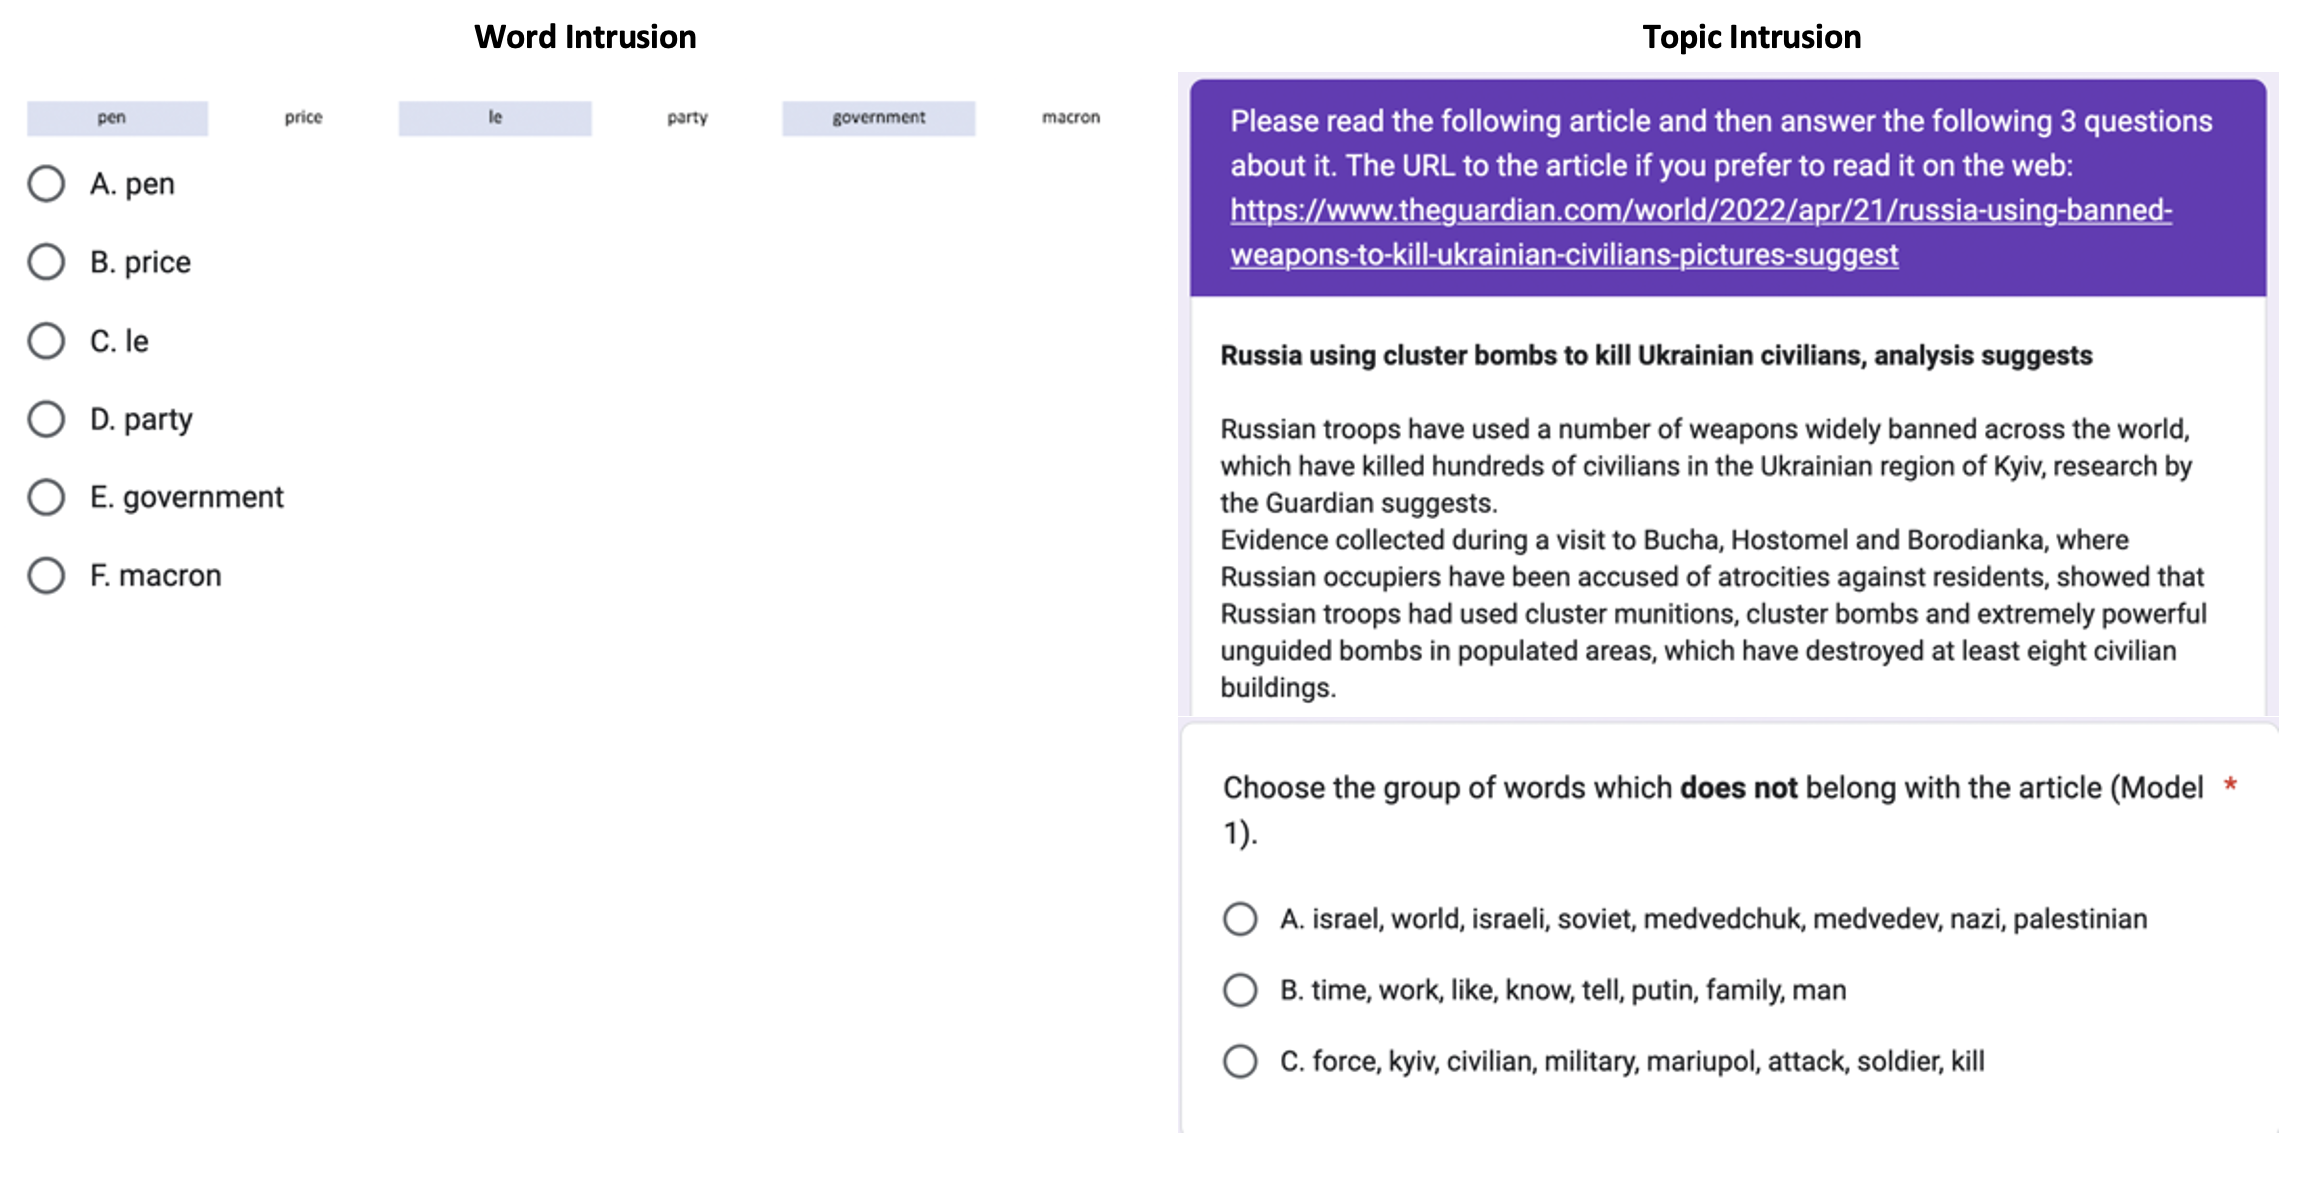
\includegraphics[scale=0.4]{forms_results.png}
\caption{\textit{Word intrusion task (left): the users are asked to select what of the words do not belong with the rest of the words. Topic intrusion task (right): the users are asked to read a news article and later is presented with 3 topics represented with their highest probable words, of which 1 of the topics does not belong to the document.}}
\label{fig:forms_results}
\end{figure}

\clearpage
\section{Results}
In Figure~\ref{fig:6_topics}, Figure~\ref{fig:8_topics}, and Figure~\ref{fig:10_topics} we can see the topics for each of the 3 models we were comparing. Each topic is represented for the 10 words with the highest probability.

In Figure~\ref{fig:charts_models} we can observe the plots of number of topics against coherence and against perplexity.

In the Table~\ref{table:forms_results} we have the results of the experiments corresponding to the human judgement tasks.\\

\begin{table}[h!]
\centering
\begin{tabular}{c c c c c} 
\hline
Experiment & Model & Correct Answers & Total Answers & Ratio \\ [0.5ex] 
\hline
& Model 1 & 13 & 50 & 0.260\\ 
Word intrusion & Model 2 & 10 & 50 & 0.200 \\
& Model 3 & 14 & 50 & 0.280 \\ [1ex] 
\hline
& Model 1 & 16 & 30 & 0.533 \\
Topic Intrusion & Model 2 & 17 & 30 & 0.567 \\
& Model 3 & 13 & 30 & 0.433 \\ [1ex] 
\hline
\end{tabular}
\caption{\textit{Results: word intrusion and topic intrusion experiments}}
\label{table:forms_results}
\end{table}

\hfill \break
\begin{figure}[h]
\centering
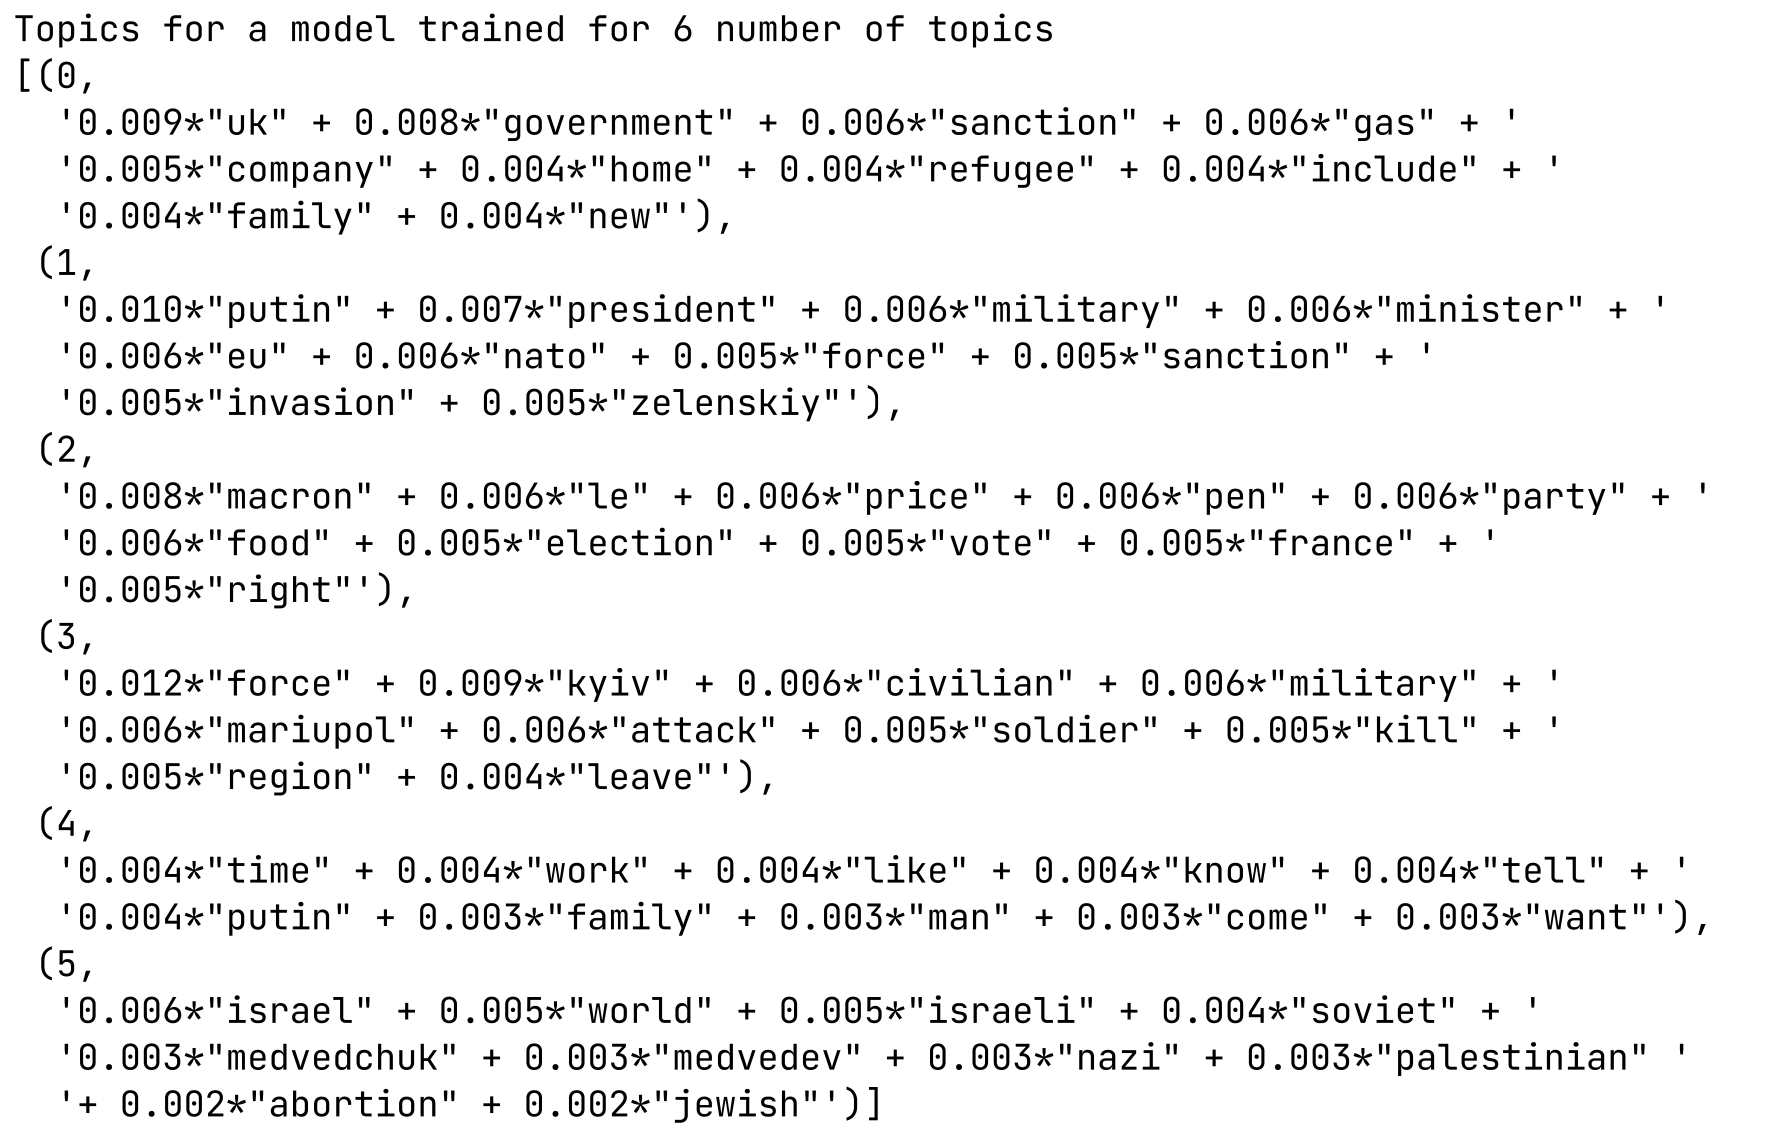
\includegraphics[scale=0.4]{6_topics.png}
\caption{\textit{Model with 6 number of topics from run 5. Each topic contains the 10 words with the highest probability within that topic.}}
\label{fig:6_topics}
\end{figure}

\begin{figure}[h]
\centering
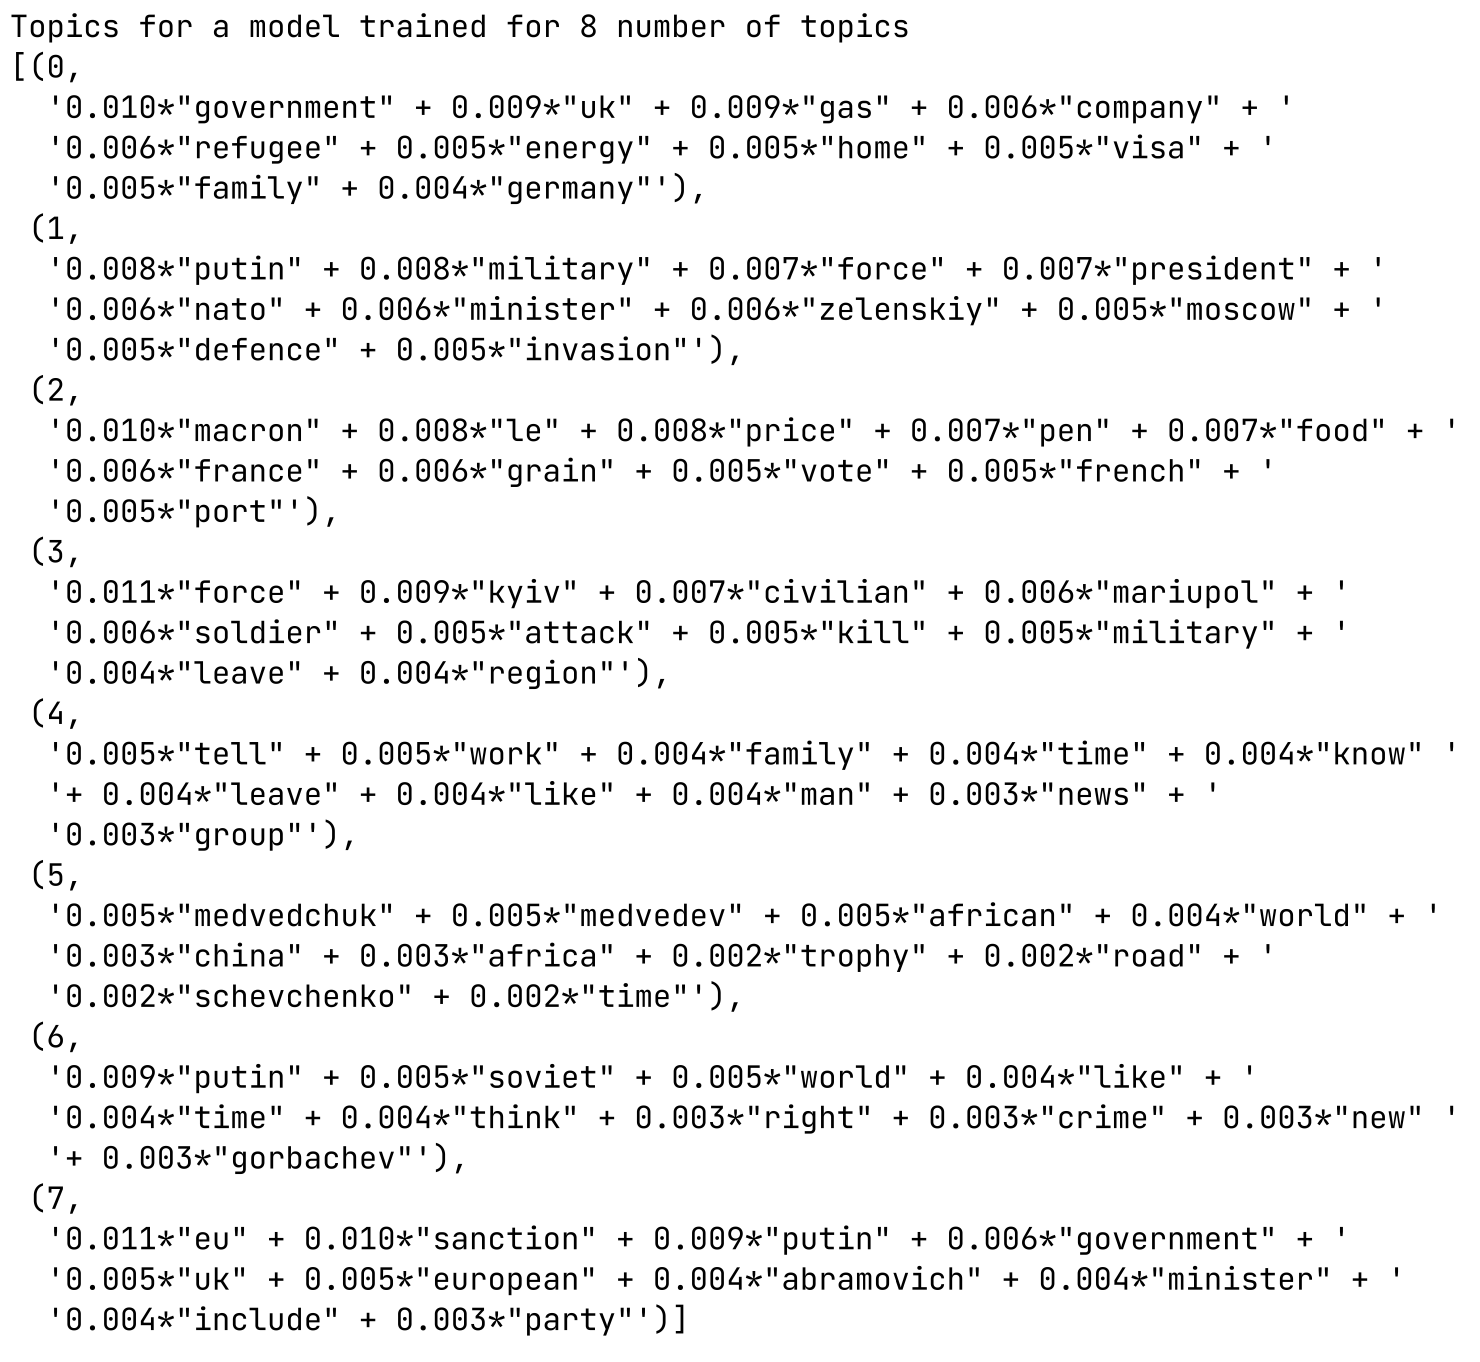
\includegraphics[scale=0.5]{8_topics.png}
\caption{\textit{Model with 8 number of topics from run 5. Each topic contains the 10 words with the highest probability within that topic.}}
\label{fig:8_topics}
\end{figure}

\begin{figure}[h]
\centering
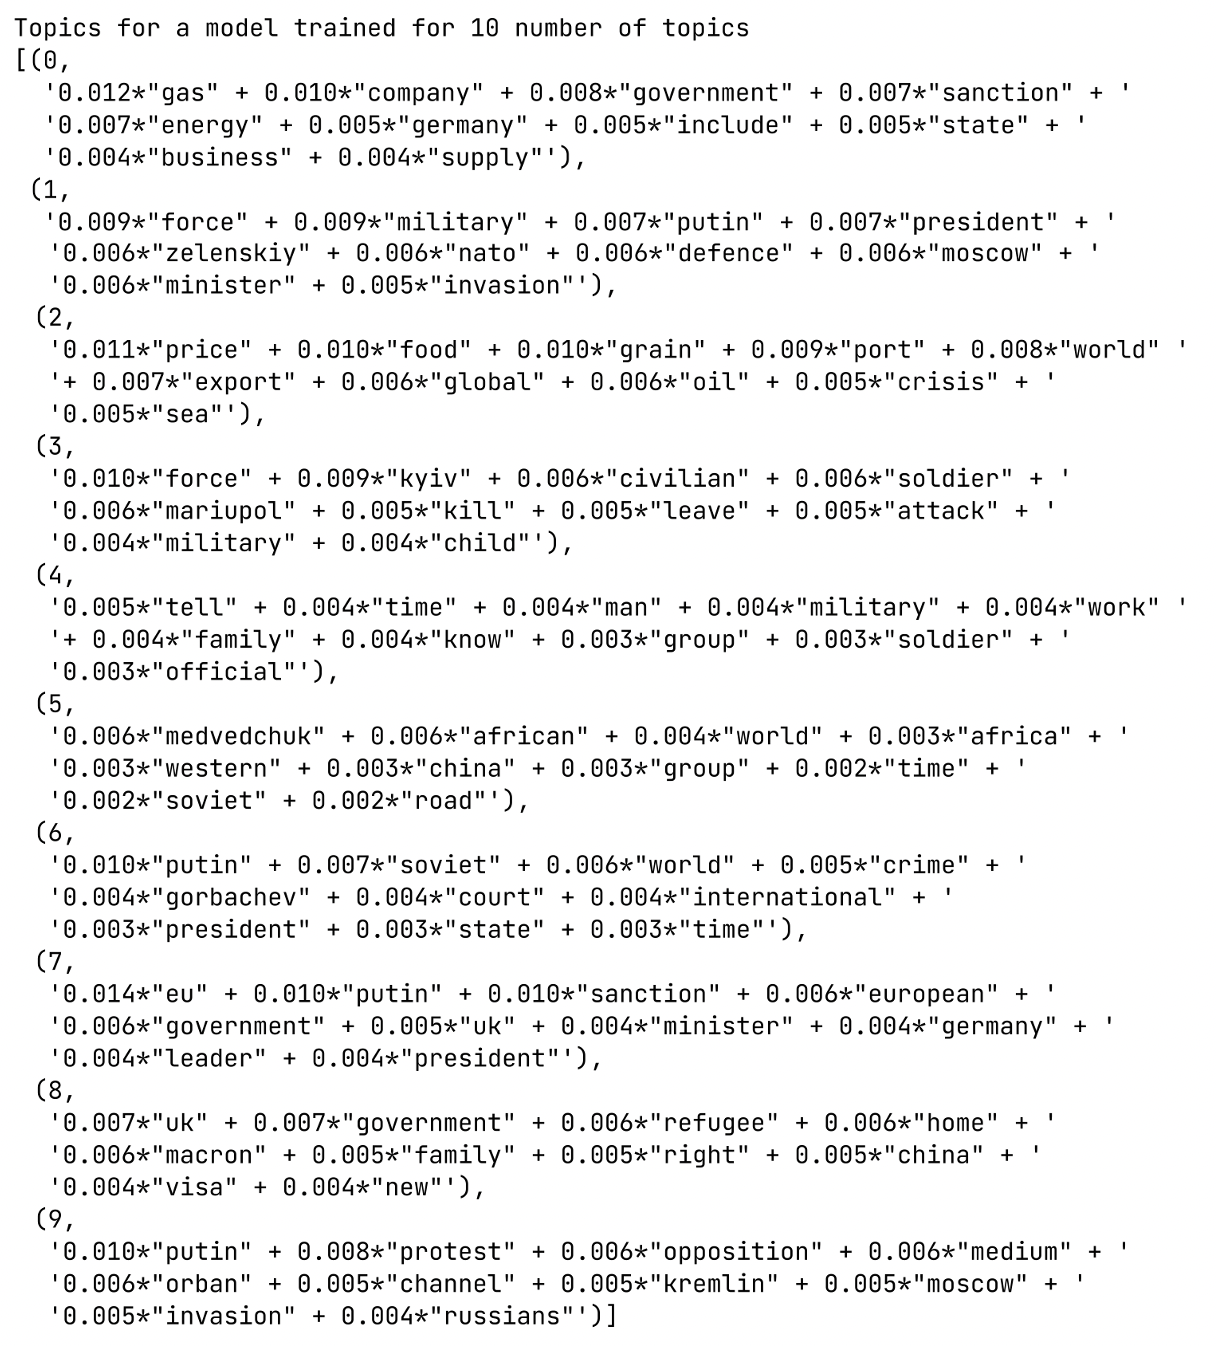
\includegraphics[scale=0.5]{10_topics.png}
\caption{\textit{Model with 10 number of topics from run 5. Each topic contains the 10 words with the highest probability within that topic.}}
\label{fig:10_topics}
\end{figure}

\begin{figure}[h]
\centering
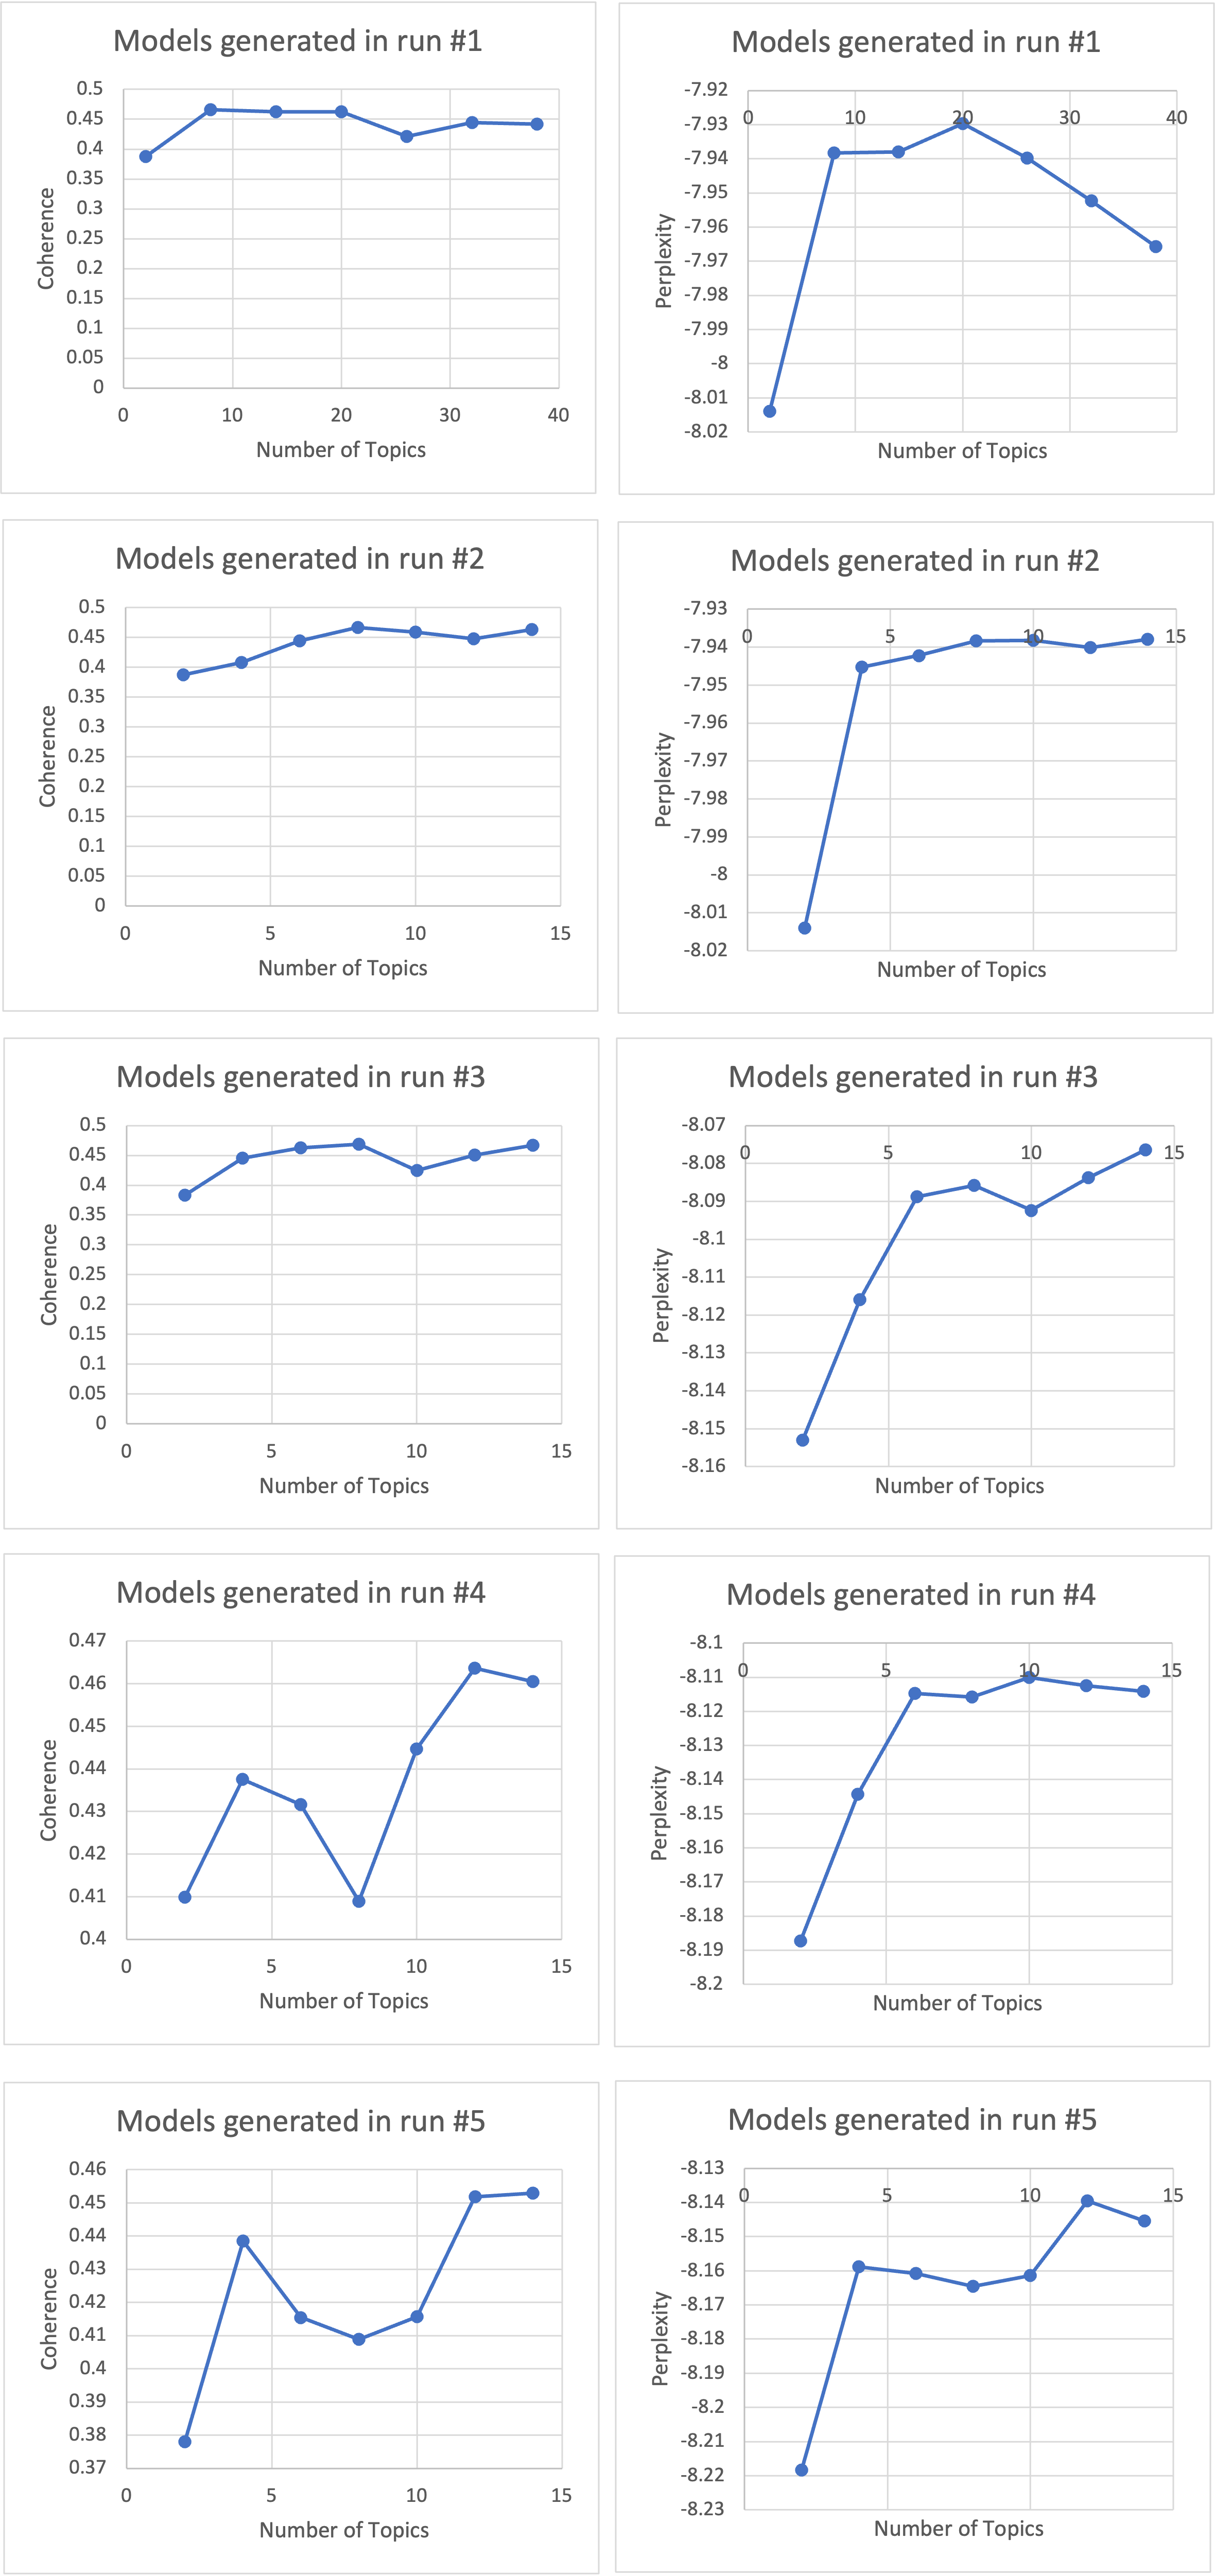
\includegraphics[scale=0.5]{charts_models.png}
\caption{\textit{Plots of coherence and perplexity for the models generated on each run during the parameter tuning process.}}
\label{fig:charts_models}
\end{figure}

\hfill \break
It can be observed that the word intrusion metric was not very decisive amongst the three models. All of the models scored low. On the other hand, Model 2 and Model 1 have a score significantly higher than the score for Model 3.

Taking into account the results from the human judgement task in addition to the analysis given by the coherence score and perplexity of our models, it can be concluded that the best model for the purposes of obtaining a general overview of our dataset through the topics is Model 2 which corresponds to a model with 8 number of topics.

In the following section we are going to discuss further the implications of selecting this model and how we can interpret the topics and what do they tell us about the current situation between Russia and Ukrania.

Additionally, to visualise the topics in an interactive way, we used pyLDAvis which is a Python library for the interactive display of topic models \citep{sievert_ldavis_2014}. In the Figure~\ref{fig:pyldavis} you can observe the visualisation of the topics for the model 2 with 8 number of topics.

\begin{figure}[h]
\centering
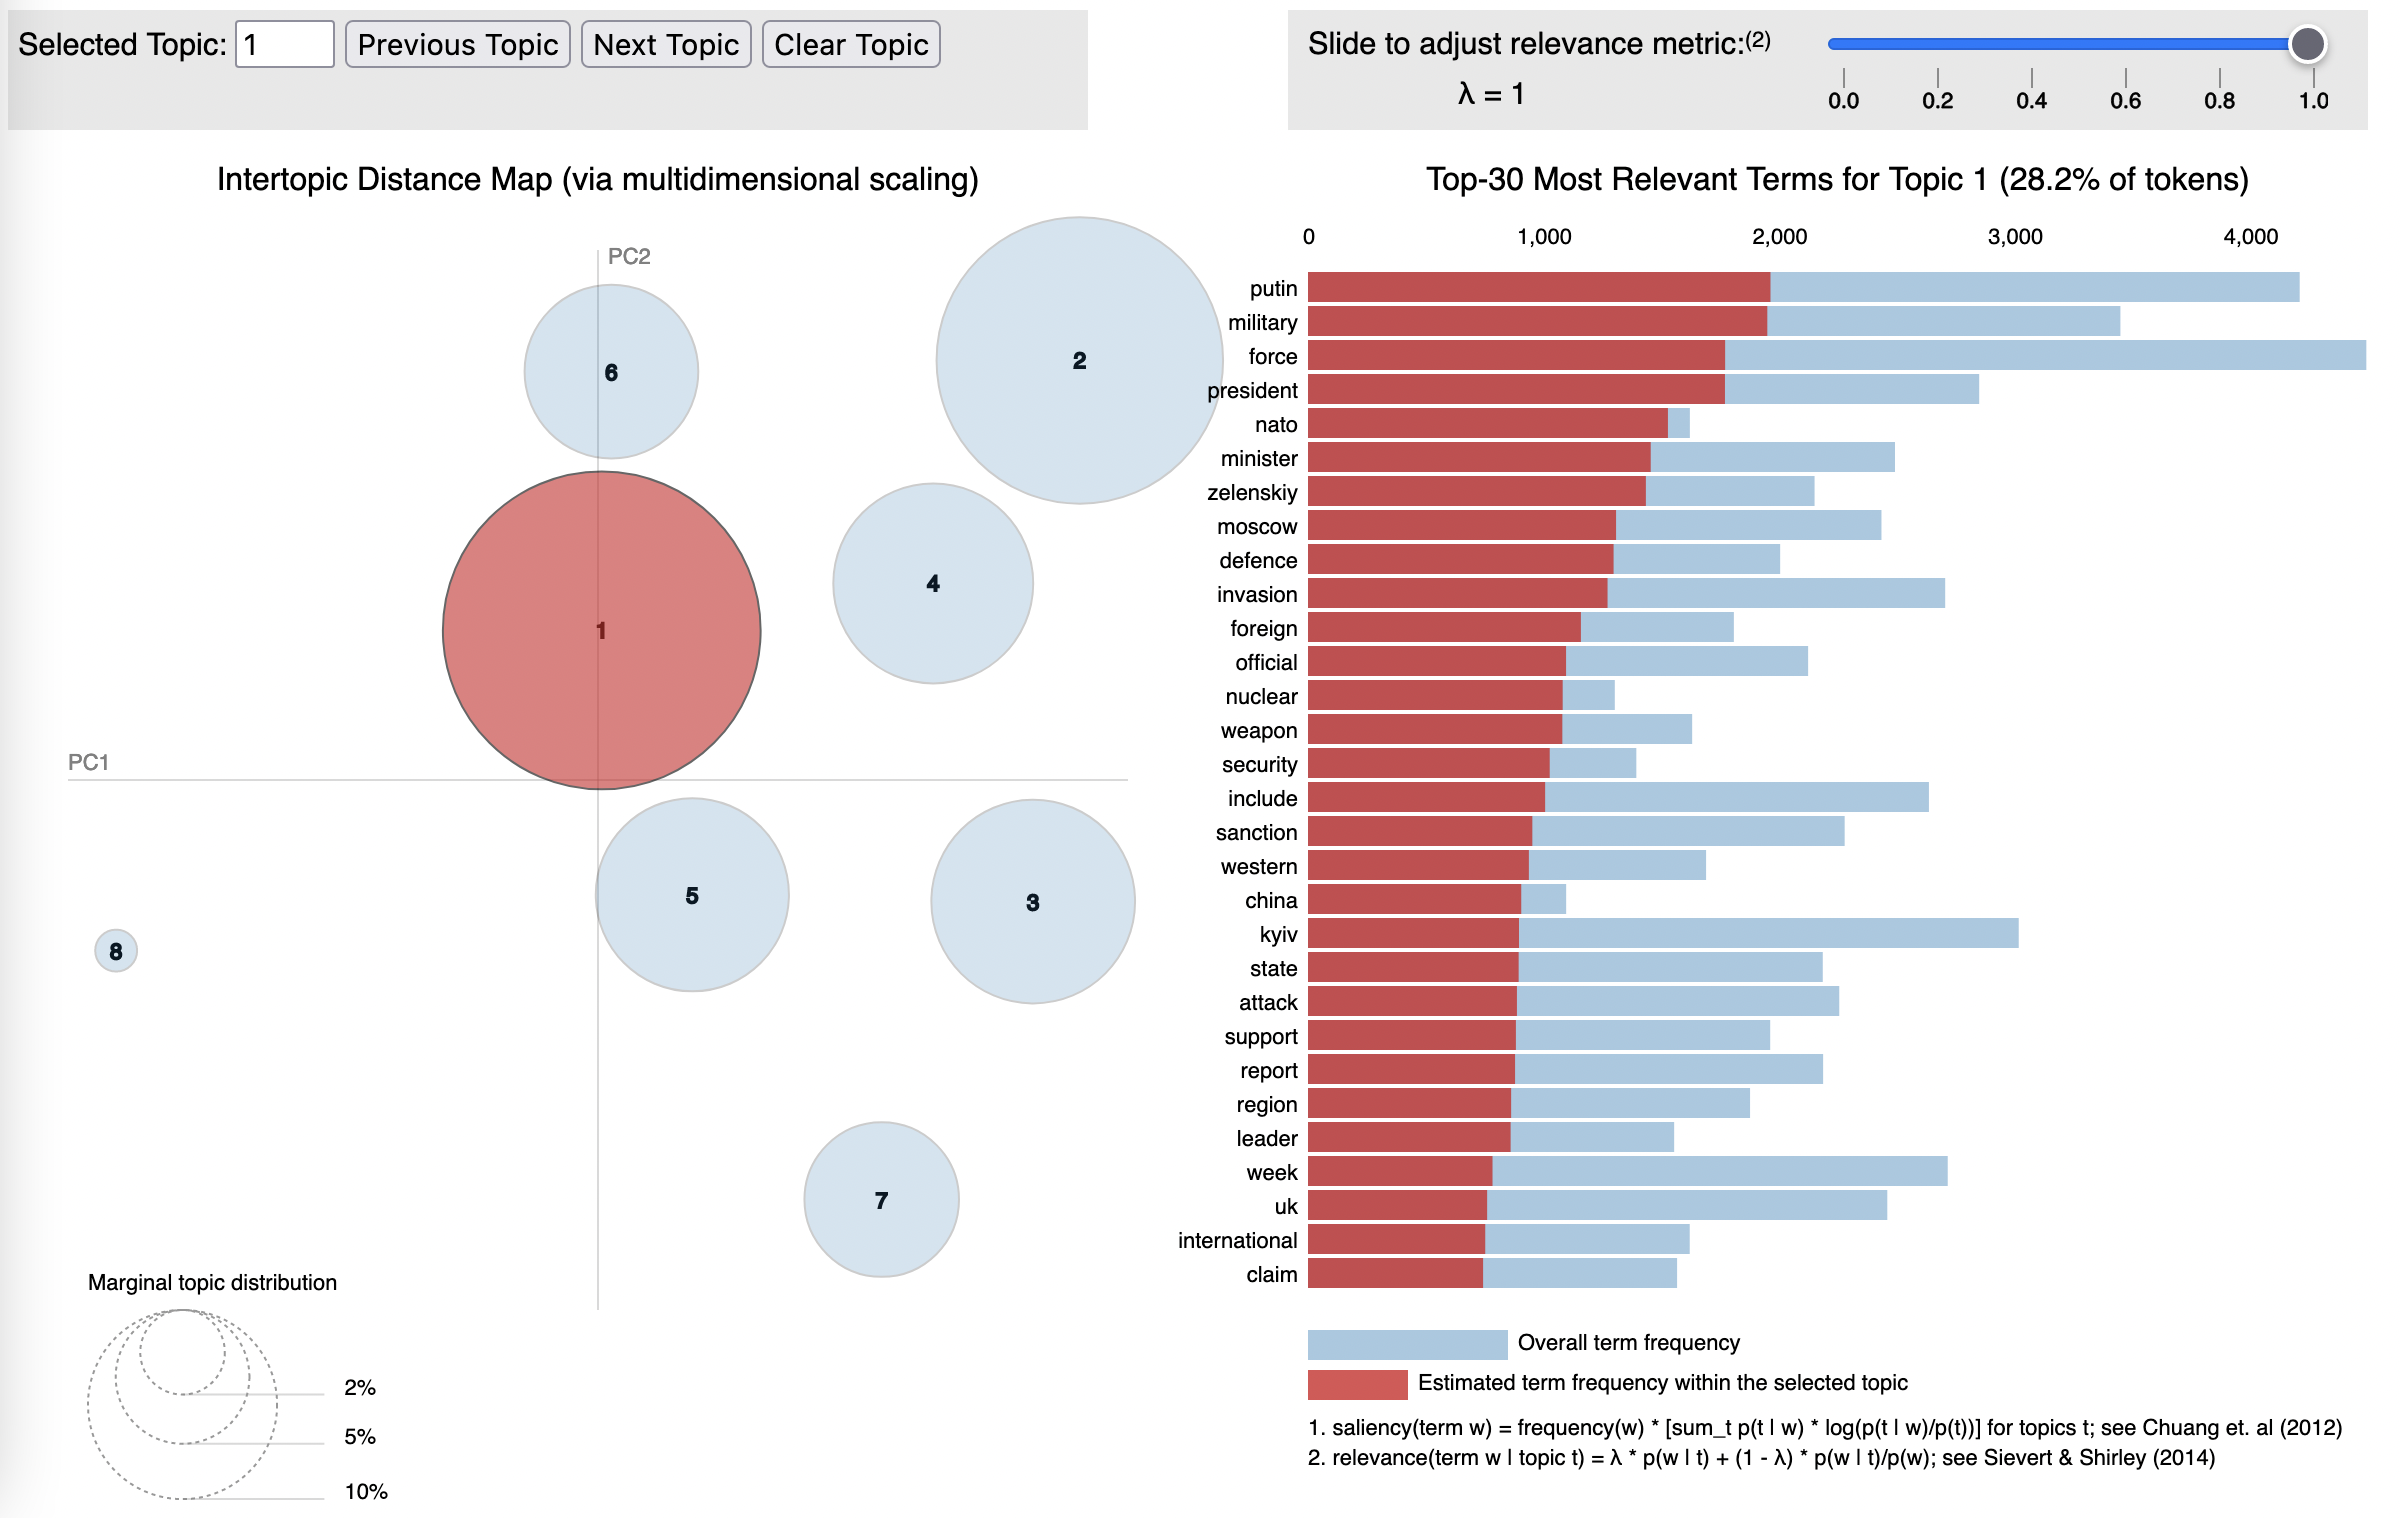
\includegraphics[scale=0.3]{pyldavis.png}
\caption{\textit{Visualisation of the topics for the model 2 which corresponds to a model with 8 number of topics. Currently showing the 30 most relevant words for topic 1.}}
\label{fig:pyldavis}
\end{figure}

\clearpage
\section{Discussion}
\subsection{Topics Interpretation}
In this section we are going to look deeper into the topics from the selected model and we are going to give an interpretation from it. This interpretation intends to give a broad idea of the current state of the conflict and the consequences that this brings for the UK and Europe.

As we can observe from Figure~\ref{fig:8_topics}, we can attempt to interpret the topics and derive ideas from them.

Topic 0 contains the words: government, uk, gas, company, refugee, energy, home, visa, family, germany.  This topic is more aimed at refugees and their worries. Like their legal status once they flee their country, their families or homes, essential things for living such as gas or energy. It could be inferred that this topic remains very present in the dataset since the news articles would be informing not only about the war but also the consequences that this is having on innocent people and how it affects their everyday life. Moreover, it could be inferred as well that the UK and Germany are receiving and helping refugees from the war.

Topic 1 contains the words: putin, military, force, president, nato, minister, zeleinskiy, moscow, defence, invasion. This topic relies heavily on the leaders of Russia and Ukraine, militia and words related to it such as defence or invasion. This topic simply demonstrates the main actors and contributors in the ongoing conflict. 

Topic 2 contains the words: macron, le, price, pen, food, france, grain, vote, french, port. This topic shows a strong relation with France and activities that have a great impact on the economy, such as food, agriculture, and imports or exports of goods. It could be said that the words on this topic indicate that this areas of the economy would be specially affected in France.

Topic 3 contains the words: force, kyiv, civilian, mariupol, soldier, attack, kill, military, leave, region. This topic relies mostly in Ukraine. It mentions two of their cities along with words that could be associated as cause and effect. For instance, an attack by the military in one of those cities would cause civilians to leave the area, leaving them without home and possibly causing a large number of refugees.

Topic 4 contains the words: tell, work, family, time, know, leave, like, man, news, group. These word are related to the day to day activities of an adult, such as work, family, time. This implies that in the dataset a great number of articles create the space to talk about how the normal life of people in both regions is being affected by the conflict. 

Topic 5 contains the words: medvedchuk, medvedev, african, world, china, africa, trophy, road, schevchenko, time. This topic contains Russian and Ukrainian names, most likely from public figures in their countries. That could mean involvement from them in the conflict. The topic also contains words related to other nations, such as China and Africa. It could be said that a good number of news articles mention how these nations, in spite of not being geographically close to the conflict as other countries, are being affected by it.

Topic 6 contains the words: putin, soviet, world, like, time, think, right, time, new, gorbachev. Names from political figures from Russia are mentioned. If we link these with the rest of the words: world, time, think, new; it could be inferred how the government or politicians are having a great influence on the decisions that are being made about the war and its impact to the world.

Topic 7 contains the words: eu, sanction, putin, government, uk, european, abramovich, minister, include, party. There are words that indicate a more general consequence for the whole continent of Europe. Politicis is included as well in words like Putin, government, minister, and party. On the other hand, it can also be inferred that Russia is being sanctioned or punished in some way by Europe as a mean to try to persuade them to stop the war.

Considering the pipeline we followed to train an LDA and then the analysis over the results to select the model that presented topics that best represented the dataset, we can...

\clearpage
\section{Conclusion}
Lorem ipsum dolor sit amet, consectetur adipiscing elit, sed do eiusmod tempor incididunt ut labore et dolore magna aliqua. Ut enim ad minim veniam, quis nostrud exercitation ullamco laboris nisi ut aliquip ex ea commodo consequat. Duis aute irure dolor in reprehenderit in voluptate velit esse cillum dolore eu fugiat nulla pariatur. Excepteur sint occaecat cupidatat non proident, sunt in culpa qui officia deserunt mollit anim id est laborum.

\clearpage
\lhead{}\chead{MSc. Project Report :: \nouppercase{\leftmark}}\rhead{}
\phantomsection
\addcontentsline{toc}{section}{References}
\bibliographystyle{agsm}
\bibliography{mybib}

\clearpage
\section{Appendix One: Accompanying Archive and Instructions}
\label{section:appendix}
\subsection{Directory Structure}
The repository can be found under the branch feature/lda-model-pycharm: \href{https://git-teaching.cs.bham.ac.uk/mod-msc-proj-2021/nfq160/-/tree/feature/lda-model-pycharm}{https://git-teaching.cs.bham.ac.uk/mod-msc-proj-2021/nfq160/-/tree/feature/lda-model-pycharm}.

The code files are under the directory "dissertation". This report files are under the directory "report". Furthermore, there is a txt file named "link to forms" which contains the url to the forms that were used for the human judgement experimentation.

\clearpage
\end{document}
